\chapter{Introdução}

Este capítulo apresenta o contexto geral no qual este trabalho está inserido, destacando a relevância dos estudos em dessalinização, o papel da destilação por membranas como tecnologia emergente e os desafios associados à modelagem de sistemas V-AGMD. Também são apresentados a motivação do estudo, seus objetivos e a organização do documento.

\section{Contextualização e Fundamentação do Problema}

A crescente escassez de recursos hídricos, impulsionada pelo crescimento populacional, urbanização e mudanças climáticas, tem intensificado a demanda por tecnologias capazes de ampliar a disponibilidade de água potável, especialmente em regiões costeiras e áreas remotas com acesso limitado a fontes convencionais de abastecimento. Nesse contexto, os processos de dessalinização vêm assumindo papel cada vez mais relevante na diversificação das matrizes hídricas, permitindo a produção de água a partir de fontes salobras ou marinhas (\cite{Elimelech2011,Shannon2008,Shemer2023}).

As tecnologias de dessalinização podem ser classificadas em duas abordagens principais: térmica e por membrana, além de métodos emergentes. As tecnologias térmicas, como a destilação por múltiplos efeitos (MED), a destilação flash multiestágios (MSF), a compressão mecânica de vapor (MVC) e a compressão térmica de vapor (TVC), baseiam-se na evaporação da água salgada e posterior condensação do vapor, produzindo água de alta qualidade, porém com elevado consumo energético (\cite{Abid2020DesalinationOverview}).

\begin{figure}[H]
    \centering
    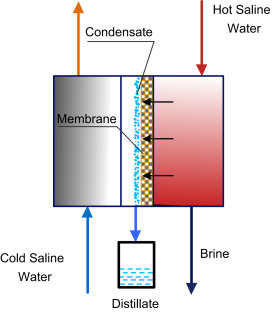
\includegraphics[width=0.8\linewidth]{Imagens/chap01/membrane.png}
    \caption[Representação esquemática do processo de dessalinização]{Representação esquemática do processo de dessalinização, no qual a água salina é submetida a um processo de separação para obtenção de água dessalinizada e de uma corrente concentrada em sais. Fonte: ...}
    \label{fig:processo_dessalinizacao}
\end{figure}

As tecnologias baseadas em membrana incluem a osmose reversa (do inglês, \textit{Reverse Osmosis} -- RO), nanofiltração (do inglês, \textit{Nanofiltration} -- NF), osmose direta (do inglês, \textit{Forward Osmosis} -- FO) e eletrodiálise (do inglês, \textit{Electrodialysis} -- ED). A RO, amplamente utilizada, emprega alta pressão para forçar a passagem de água por uma membrana semipermeável, enquanto a FO utiliza gradientes osmóticos e a ED campos elétricos para separação iônica. Alternativamente, a dessalinização por congelamento (do inglês, \textit{Freeze Desalination} -- FD) promove a separação da água na forma de cristais de gelo. A escolha da tecnologia depende de fatores como qualidade da água de alimentação, demanda energética e custos operacionais (\cite{Abid2020DesalinationOverview}).

Nesse contexto, a destilação por membrana (do inglês, \textit{Membrane Distillation} -- MD) destaca-se como um processo híbrido que combina princípios térmicos e de separação por membranas. A MD baseia-se na migração de vapor de água através de uma membrana hidrofóbica, impulsionada por uma diferença de pressão de vapor induzida por gradiente de temperatura, resultando em elevada rejeição de sais (\cite{Abid2020DesalinationOverview,Cath2010}).

A MD apresenta vantagens como operação em condições moderadas de temperatura e pressão, possibilidade de uso de fontes térmicas de baixa qualidade ou calor residual, e aplicabilidade em soluções de alta salinidade. Exemplos dessas fontes incluem sistemas de dessalinização alimentados por energia solar térmica, unidades integradas a calor residual proveniente de processos industriais, usinas de energia e sistemas marítimos, bem como o uso de energia geotérmica e configurações híbridas com recuperação de calor. Estudos também reportam o desenvolvimento de unidades piloto de MD alimentadas por energia solar, evidenciando a viabilidade técnica e econômica dessas integrações (\cite{Yadav2021MDLowGradeEnergy}). Além disso, avanços recentes, como integração com fontes renováveis, recuperação de calor latente e desenvolvimento de módulos escaláveis, têm reforçado seu potencial para aplicações em larga escala, destacando a importância da modelagem para o projeto e otimização desses sistemas (\cite{Cath2010,Leaper2021,Warsinger2017,Parani2021,AndresManas2022}).

Diferentes configurações de MD foram desenvolvidas, distinguindo-se principalmente pelos mecanismos de transporte de vapor e pelas estratégias de condensação/coleta do permeado. Entre as principais configurações, destacam-se a destilação por membrana de contato direto (do inglês, \textit{Direct Contact Membrane Distillation} -- DCMD), na qual o vapor gerado na alimentação quente atravessa a membrana e condensa diretamente em uma corrente fria em contato com o permeado; a destilação por membrana com gás de varredura (do inglês, \textit{Sweeping Gas Membrane Distillation} -- SGMD), em que um gás de arraste remove o vapor do lado do permeado e o conduz a um condensador externo; e a destilação por membrana a vácuo (do inglês, \textit{Vacuum Membrane Distillation} -- VMD), na qual a aplicação de vácuo parcial no lado do permeado intensifica o transporte de vapor, sendo este posteriormente condensado fora do módulo.

A configuração de destilação por membrana com lacuna de ar (do inglês, \textit{Air Gap Membrane Distillation} -- AGMD) se destaca pela presença de uma camada de ar entre a membrana e a superfície de condensação, que reduz perdas térmicas por condução, mas introduz resistência ao transporte de massa. Essa resistência adicional aumenta o caminho difusivo do vapor e, consequentemente, reduz o fluxo de permeado em comparação a outras configurações, como DCMD e VMD, evidenciando um compromisso entre eficiência térmica e taxa de produção de água dessalinizada (\cite{AlZoubi2018,Chong2022,Abid2020DesalinationOverview}).

Uma evolução dessa configuração é a destilação por membrana com lacuna de ar aprimorada por vácuo (do inglês, \textit{Vacuum-Enhanced Air Gap Membrane Distillation} -- V-AGMD), na qual a aplicação de pressão reduzida no espaço de ar diminui a resistência ao transporte de vapor, aumentando o fluxo de permeado, ao mesmo tempo em que mantém o isolamento térmico proporcionado pela presença da camada de ar. Essa configuração apresenta potencial promissor, especialmente quando associada a fontes de calor de baixa qualidade (\cite{Warsinger2017,Zewdie2020}).

O desempenho de sistemas V-AGMD depende fortemente de variáveis operacionais, como as temperaturas de entrada das correntes de alimentação e de resfriamento, a salinidade da alimentação, as vazões e a pressão no espaço de ar. No processo MD, os fenômenos de transferência de calor e massa ocorrem de forma simultânea e acoplada: o gradiente térmico determina a diferença de pressão de vapor que impulsiona o transporte de massa, enquanto a evaporação e a condensação alteram os fluxos de calor no módulo. Além disso, a salinidade, a vazão e o nível de vácuo afetam as resistências ao transporte e a força motriz do processo. Dessa forma, a resposta do sistema resulta da interação entre múltiplas variáveis operacionais, tornando desafiadora a previsão simultânea do fluxo de permeado e das temperaturas de saída das correntes de alimentação e de resfriamento. A estimativa adequada dessas temperaturas é particularmente relevante, pois elas podem ser utilizadas no cálculo de indicadores de desempenho energético, como o consumo específico de energia (SEC) e o ganho de saída (GOR) (\cite{Hitsov2015,Olatunji2018}).

De modo geral, a modelagem de sistemas de destilação por membranas pode seguir duas abordagens principais: modelos físico-matemáticos e modelos baseados em dados experimentais. Os modelos físico-matemáticos representam o processo a partir de balanços de massa e energia, relações termodinâmicas e mecanismos de transferência de calor e massa. Por isso, apresentam elevada interpretabilidade física e consistência termodinâmica, embora frequentemente exijam simplificações estruturais ou elevado esforço computacional (\cite{Hitsov2015,Olatunji2018}). Por outro lado, os modelos baseados em dados experimentais utilizam medições do sistema para aprender relações entre variáveis operacionais e variáveis de desempenho, por meio de técnicas como regressão e redes neurais artificiais. Esses modelos podem capturar relações complexas sem exigir a formulação explícita de todos os fenômenos envolvidos, mas dependem fortemente da disponibilidade, representatividade e qualidade dos dados experimentais utilizados no treinamento (\cite{Zhu2022}).

Para os modelos baseados em dados experimentais, a obtenção de observações em sistemas reais é frequentemente limitada e onerosa, o que torna a capacidade de generalização um desafio central. Nesse contexto, modelos de maior complexidade, isto é, modelos com maior capacidade de adaptação aos dados de treinamento, podem apresentar bom desempenho durante o ajuste, mas falhar quando aplicados a novas condições operacionais. Essa complexidade pode estar associada, por exemplo, ao número de parâmetros do modelo, à profundidade de árvores, à quantidade de camadas ou neurônios em redes neurais e ao grau de regularização adotado. Além disso, a avaliação baseada apenas em métricas médias pode mascarar instabilidades associadas à variabilidade dos dados e das partições de validação, tornando essencial a adoção de estratégias robustas de validação (\cite{Vabalas2019,Yip2019,Roberts2017,Kirk2024}).

Diante dessas limitações, abordagens híbridas de modelagem têm emergido como uma alternativa promissora, combinando modelos físico-matemáticos com técnicas baseadas em dados. A incorporação de conhecimento físico no processo de aprendizado pode restringir o espaço de soluções admissíveis, reduzir a dependência de grandes volumes de dados e melhorar a capacidade de generalização dos modelos (\cite{Xu2022,Muther2022,Kasilingam2024}).

Nesse contexto, torna-se necessária a adoção de uma abordagem metodológica estruturada para a avaliação e seleção de modelos de regressão supervisionada aplicados ao processo V-AGMD, considerando simultaneamente a natureza não linear do sistema, as limitações do conjunto de dados disponível e o potencial de integração entre conhecimento físico e aprendizado baseado em dados.

\section{Motivação}

O presente trabalho está inserido no contexto das atividades desenvolvidas no Laboratório de Micro e Nanofluídica e Microssistemas (LabMEMS) da Universidade Federal do Rio de Janeiro (UFRJ), no âmbito de um projeto multidisciplinar voltado à cogeração sustentável de energia elétrica e produção de água potável a partir do aproveitamento de energia solar térmica. Nesse sistema, painéis solares são utilizados para aquecer a corrente de alimentação de uma unidade piloto de destilação por membranas, disponível comercialmente, com capacidade de operação nas configurações AGMD e V-AGMD, permitindo integrar geração de energia e dessalinização em uma mesma planta experimental.

A motivação deste estudo decorre da necessidade de compreender e prever o desempenho dessa planta de cogeração, especialmente no módulo de dessalinização por membranas operado na configuração V-AGMD, na qual há presença de espaço de ar e aplicação de vácuo parcial. O sistema experimental fornece dados reais obtidos sob diferentes regimes operacionais, nos quais variáveis como temperaturas de entrada, vazões, salinidade e nível de vácuo parcial influenciam simultaneamente o fluxo de permeado e as temperaturas de saída das correntes. A previsão dessas grandezas é relevante tanto para avaliar a produção de água dessalinizada quanto para estimar indicadores energéticos associados ao processo.

Além dos dados experimentais, foi utilizado como referência comparativa um modelo físico-matemático reduzido do tipo 0D, previamente descrito na literatura para esse sistema (\cite{Lisboa2024}). A disponibilidade simultânea de dados reais da planta de cogeração e de um modelo físico reduzido permite investigar estratégias de modelagem baseadas em dados e abordagens híbridas, nas quais informações provenientes da física do processo podem complementar o aprendizado dos modelos.

Dessa forma, a motivação central deste trabalho está na necessidade de avaliar ferramentas preditivas capazes de representar o desempenho de sistemas V-AGMD a partir de dados experimentais limitados, explorando simultaneamente o potencial de modelos baseados em dados e de estratégias híbridas que incorporam conhecimento físico. Assim, o estudo busca contribuir para a análise, operação e futura otimização de sistemas V-AGMD integrados a fontes renováveis de energia.

\section{Objetivos}

\subsection{Objetivo geral}

O objetivo geral deste trabalho é avaliar estratégias de modelagem baseada em dados e modelagem híbrida físico--dados para a predição do desempenho de um sistema de destilação por membranas do tipo V-AGMD, considerando como variáveis de saída o fluxo de permeado e as temperaturas de saída das correntes de alimentação e resfriamento.

\subsection{Objetivos específicos}

Para atingir o objetivo geral, são definidos os seguintes objetivos específicos:

\begin{itemize}
    \item estruturar a base de dados experimental do sistema V-AGMD, definindo variáveis de entrada, variáveis de saída e agrupamentos por regime operacional;

    \item avaliar o desempenho de um modelo físico reduzido 0D como referência comparativa para as variáveis de saída do sistema;

    \item comparar diferentes famílias de modelos de regressão supervisionada, incluindo modelos lineares, modelos baseados em árvores, redes neurais artificiais e arquiteturas híbridas;

    \item aplicar uma estratégia de validação cruzada por grupos, considerando a separação entre regimes experimentais, de modo a avaliar a capacidade de generalização dos modelos;

    \item selecionar o modelo final com base em critérios de desempenho preditivo, diferença de generalização e complexidade estrutural;

    \item analisar o potencial da incorporação de informações físicas na melhoria do desempenho de modelos baseados em dados para a predição do processo V-AGMD.
\end{itemize}

\section{Organização do TCC}

Este trabalho está organizado em seis capítulos. O Capítulo 1 apresenta a introdução, incluindo a contextualização do problema, a motivação do estudo, os objetivos e a organização do documento.

O Capítulo 2 apresenta a revisão bibliográfica sobre a modelagem de sistemas de destilação por membranas, abordando modelos baseados em primeiros princípios, modelos orientados por dados, estratégias híbridas e lacunas da literatura.

O Capítulo 3 reúne a fundamentação teórica necessária ao trabalho, incluindo os princípios da destilação por membranas, o modelo físico reduzido utilizado como referência e os conceitos de aprendizado de máquinas aplicados à regressão.

O Capítulo 4 descreve a metodologia proposta, contemplando a preparação dos dados, a validação cruzada, os critérios de seleção, as famílias de modelos avaliadas e as estratégias de integração com o modelo físico.

O Capítulo 5 apresenta os resultados, incluindo a análise exploratória dos dados, a avaliação do modelo físico reduzido, a comparação entre modelos baseados em dados e a seleção do modelo final.

Por fim, o Capítulo 6 apresenta as conclusões do trabalho e sugestões para pesquisas futuras.